%%%%%%%%%%%%%%%%%%%%%%%%%%%%%%%%%%%%%%%%%
% Beamer Presentation
% LaTeX Template
% Version 1.0 (10/11/12)
%
% This template has been downloaded from:
% http://www.LaTeXTemplates.com
%
% License:
% CC BY-NC-SA 3.0 (http://creativecommons.org/licenses/by-nc-sa/3.0/)
%
%%%%%%%%%%%%%%%%%%%%%%%%%%%%%%%%%%%%%%%%%

%----------------------------------------------------------------------------------------
%	PACKAGES AND THEMES
%----------------------------------------------------------------------------------------

\documentclass{beamer}

%\documentclass[aspectratio=169]{beamer}

\mode<presentation> {

% The Beamer class comes with a number of default slide themes
% which change the colors and layouts of slides. Below this is a list
% of all the themes, uncomment each in turn to see what they look like.

%\usetheme{default}
%\usetheme{AnnArbor}
%\usetheme{Antibes}
%\usetheme{Bergen}
%\usetheme{Berkeley}
%\usetheme{Berlin}
%\usetheme{Boadilla}
%\usetheme{CambridgeUS}
%\usetheme{Copenhagen}
%\usetheme{Darmstadt}
%\usetheme{Dresden}
%\usetheme{Frankfurt}
%\usetheme{Goettingen}
%\usetheme{Hannover}
%\usetheme{Ilmenau}
%\usetheme{JuanLesPins}
%\usetheme{Luebeck}
\usetheme{Madrid}
%\usetheme{Malmoe}
%\usetheme{Marburg}
%\usetheme{Montpellier}
%\usetheme{PaloAlto}
%\usetheme{Pittsburgh}
%\usetheme{Rochester}
%\usetheme{Singapore}
%\usetheme{Szeged}
%\usetheme{Warsaw}

% As well as themes, the Beamer class has a number of color themes
% for any slide theme. Uncomment each of these in turn to see how it
% changes the colors of your current slide theme.

%\usecolortheme{albatross}
%\usecolortheme{beaver}
%\usecolortheme{beetle}
%\usecolortheme{crane}
%\usecolortheme{dolphin}
%\usecolortheme{dove}
%\usecolortheme{fly}
%\usecolortheme{lily}
%\usecolortheme{orchid}
%\usecolortheme{rose}
%\usecolortheme{seagull}
%\usecolortheme{seahorse}
%\usecolortheme{whale}
%\usecolortheme{wolverine}

%\setbeamertemplate{footline} % To remove the footer line in all slides uncomment this line
%\setbeamertemplate{footline}[page number] % To replace the footer line in all slides with a simple slide count uncomment this line

%\setbeamertemplate{navigation symbols}{} % To remove the navigation symbols from the bottom of all slides uncomment this line
}

\usepackage[spanish]{babel}
\usepackage[utf8]{inputenc}
\usepackage{amsmath, amssymb}
\usepackage{hyperref}
\usepackage{geometry}
\usepackage{graphicx} % Allows including images
\usepackage{booktabs} % Allows the use of \toprule, \midrule and \bottomrule in tables

%----------------------------------------------------------------------------------------
%	TITLE PAGE
%----------------------------------------------------------------------------------------

\title[\LaTeXe]{Introducción básica a \LaTeX} % The short title appears at the bottom of every slide, the full title is only on the title page

\author{Fernando Oleo Blanco} % Your name
\institute[ICAI] % Your institution as it will appear on the bottom of every slide, may be shorthand to save space
{
Universidad ICAI Comillas \\ % Your institution for the title page
Asociación de LinuxEC \\
\medskip
\textit{201507027@alu.comillas.edu} % Your email address
}
\date % Date, can be changed to a custom date

\begin{document}

\begin{frame}
\titlepage % Print the title page as the first slide
\end{frame}

\begin{frame}
\frametitle{Organización} % Table of contents slide, comment this block out to remove it

\begin{enumerate}
	\item Primera Charla: Introducción general básica
	\begin{itemize}
		\item Comparativa con MS Word
		\item Descarga e instalación
		\item Introducción \textit{histórica} de \LaTeX
		\item Documento básico, estructura de un comando y buenas prácticas
		\item Herramientas básicas
		\item Entornos
	\end{itemize}
	\item Segunda Parte: entorno de presentaciones Beamer
	\item Tercera Sesión: herramientas de escritura científica
	\begin{itemize}
		\item Más entornos: \textit{in line, array, equation...}
		\item \texttt{Amsmath}
		\item Tikz \\
		$\vdots$
	\end{itemize}
\end{enumerate}

\end{frame}

\begin{frame}{Recursos recomendados}
\begin{block}{Lectura}
	$\bullet$ \href{https://tobi.oetiker.ch/lshort/lshort.pdf}{\textit{The not so Short Introduction to \LaTeX}} por Tobias Oetiker \\
	$\bullet$ \href{https://en.wikibooks.org/wiki/LaTeX}{\textit{\LaTeX\ Wikibook:}} Libro escrito por y para Wikipedia \\
	$\bullet$ \href{http://osl.ugr.es/CTAN/info/Math_into_LaTeX-4/Short_Course.pdf}{\textit{More Math Into \LaTeX}} por George Grätzner (esta es una buena muestra)
\end{block}
\begin{block}{Internet}
	$\bullet$ \href{https://www.overleaf.com/}{\textbf{Overleaf:}} escritura de \LaTeX en el navegador $\leftarrow$ ya os estáis metiendo \\
	$\bullet$ Cualquier servicio con plantillas (\href{http://www.latextemplates.com/}{\textbf{Latextemplates}} por ejemplo) \\
	$\bullet$ \href{https://www.tug.org/begin.html}{\textbf{Tug:}} Centro de recursos \textit{oficiales} \\
	$\bullet$ \href{https://es.sharelatex.com/learn/}{Foros}, "puntos de información", etc \\
	$\bullet$ Google
\end{block}

\end{frame}

\begin{frame}
	Hoy: Una hora y media...
	\tableofcontents
\end{frame}

%----------------------------------------------------------------------------------------
%	PRESENTATION SLIDES
%----------------------------------------------------------------------------------------

%------------------------------------------------
\section{Introducción} % Sections can be created in order to organize your presentation into discrete blocks, all sections and subsections are automatically printed in the table of contents as an overview of the talk
%------------------------------------------------

\subsection{\LaTeXe\ y MS Word} % A subsection can be created just before a set of slides with a common theme to further break down your presentation into chunks

\begin{frame}
\frametitle{\LaTeX\ es... Anarka...}
M\$ Word:
\begin{itemize}
	\item Muy sencillo y simple. Las herramientas básicas son bien sencillas de utilizar (imágenes, tablas, gráficas...). Son las \textbf{únicas} que usáis.
	\item Creación de gráficos y tablas con Exel (potente) y de presentaciones con PowerPoint
	\item Bastante fácil de usar en grupo. \textit{Portátil y conocido}
\end{itemize}
\LaTeX: eso...
\begin{itemize}
	\item Complicado, poco conocido
	\item Solo para los científicos
	\item Material usado en ruedas de aviones y otras utilidades
	\item Google se hartará de tus dudas
\end{itemize}
\end{frame}

\begin{frame}
\frametitle{\LaTeX\ es... Anarka...}
M\$ Word:
\begin{itemize}
	\item \textbf{Trabajo en equipo:} Tú en Arial 12, yo en Time New Roman 12 y Pedro en Calibri 16, que ha de ocupar una cara
	\item \textbf{Profesionalidad} es cuadrar un gráfico a mano y dar formato a una tabla a como paguen
	\item Pagas por tener herramientas como fondos de gotas y títulos de arcoíris
\end{itemize}
\LaTeXe
\begin{itemize}
	\item Multiplataforma (Windows, OSX, Linux, BSDs, Solaris). Gratis.
	\item Perfectamente estructurado. Se diferencian a simple vista
	\item Muy profesional. Aunque requiere mucho aprendizaje
	\item Opciones por defecto sanas
	\item Automatización absoluta. Similar a lenguajes de programación (\texttt{html, markdown, etc}) tanto en forma como en flexibilidad
\end{itemize}
\end{frame}

%------------------------------------------------

\begin{frame}[fragile]
\frametitle{\LaTeX\ es... Anarka...}
En la práctica:
\begin{itemize}
	\item \textbf{Tablas:} mucho más fáciles de crear en Word. Pero el formato es mucho más sencillo y potente en \LaTeX
	\item \textbf{Imágnes:} sencillas de manejar en Word. Estructura definida en \LaTeX, además de ser más limpias y referenciables 
	\item \textbf{Plantillas:} \LaTeX\ es reutilizable, y se recomienda esta práctica. Word... eh...
	\item \textbf{Índices y bibliografías} automáticas y limpias
	\item Los documentos se pueden partir: \verb|\include{file}|
	\item Portátil, editores gratis, archivos de salida en \texttt{pdf}
	\item \textit{Único} paquete para escribir documentos científicos
\end{itemize}
$\bullet$ Word para trabajos sencillos y rápidos. \LaTeX\ para trabajos formales y largos
\end{frame}

\subsection{¿Quién usa \LaTeX?}

\begin{frame}
	\frametitle{¿Quién usa \LaTeX?}
	\centering Como esta charla no tratara temas científicos...
	\vspace{-10px}
	\begin{columns}[c]
		\column{0.5\textwidth}
		\begin{figure}
			\centering
			
\includegraphics[width=0.6\textwidth]{images/Fg_wings_large}
		\end{figure}
		\vspace{-35px}
		\begin{figure}
			\centering
			
\includegraphics[width=0.6\linewidth]{images/Springer-logo-logotype}
		\end{figure}
		\vspace{-35pt}
		\begin{figure}
			\centering
			
\includegraphics[width=0.6\linewidth]{images/freebsd}
		\end{figure} \pause
		\column{0.5\textwidth}
		\vspace{10px}
		\begin{figure}
			\centering
			
\includegraphics[width=0.7\linewidth]{images/patrick-bateman-business-card-scene-american-psycho}
			\caption{Patrik Bateman}
		\end{figure}
	\end{columns}
\end{frame}

%------------------------------------------------
\subsection{Instalación}

\begin{frame}
\frametitle{Instalación}

\begin{block}{TexStudio}
$\bullet$ \href{http://www.texstudio.org/}{\textbf{\TeX Studio:}} Download $\rightarrow$ busca tu plataforma. Instálalo como solo tú sabes
\end{block}

\begin{block}{TexLive}
$\bullet$ \href{https://www.tug.org/texlive/}{\textbf{Tug}} \\
Windows: download e instaláis, instaláis \textbf{todo} 4.5Gb \\
Mac: Link MacTeX distribution. Instaláis y listo
\end{block}

\begin{block}{Listo}
Listo
\end{block}
\end{frame}

%------------------------------------------------

\subsection{Donald Ervin Knuth}
\begin{figure}
	\centering
	\vspace*{10px}
	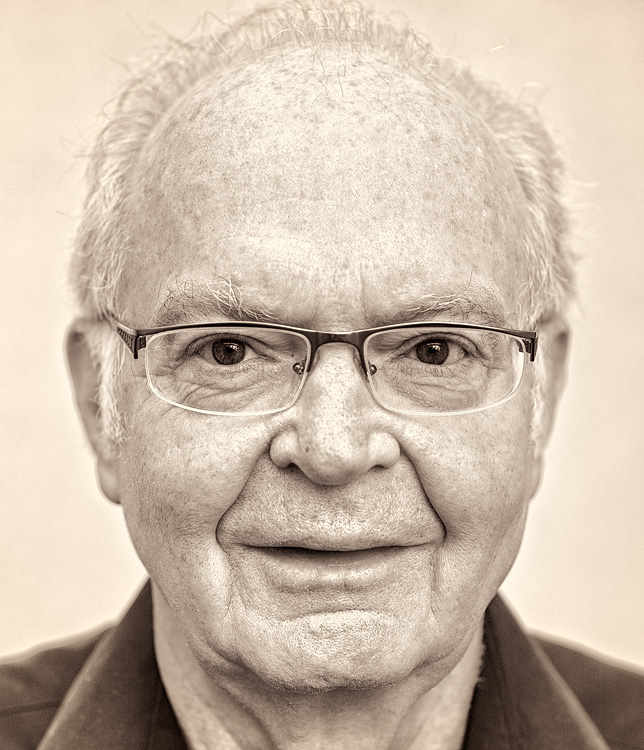
\includegraphics[height=0.6\linewidth]{images/Donald-Knuth-Stanford-Computer-Science}
	\caption{Donald Ervin Knuth. Creador de \TeX}
	\label{fig:donald-knuth-stanford-computer-science}
\end{figure}

\begin{frame}
\frametitle{Un pequeño cuento}
\begin{block}{¿Quién es Knuth?}
	Americano. Profesor de Stanford, ya retirado. Matemático, físico, informático y teólogo. Actualmente escribe la serie de libros \texttt{The Art of Computer Programming,} precursora del nacimiento de \TeX. Considerado uno de los padres de la informática moderna
\end{block}

\begin{block}{\TeX}
	Después de crear el segundo volumen y empezar el tercero se dio cuenta que la tipografía carecía calidad. Buscó soluciones y decidió estudiar tipografía para crearse su propio sistema. \TeX es el entorno de programación, \LaTeX\ es \TeX\ y unos paquetes para agilizar su escritura
\end{block}

\begin{block}{Curiosidades}
	\textit{"Si una herramienta que uso la utilizan muchas personas, seguramente pensaría que estoy haciendo algo mal"}
\end{block}
\end{frame}

%-------------------------------------------------------------------------------

\section{Introducción al editor}

\begin{frame}
	\frametitle{TexStudio}
	Comprueba la hora. \\
	Venga Fer, que tu puedes.
\end{frame}

%-------------------------------------------------------------------------------

\section{Documento básico de \LaTeX}

\begin{frame}[fragile]
	\frametitle{Consejos}
	Procedimiento que \textbf{simpre, siempre, siempre} seguiréis
	\begin{itemize}
		\item Nunca empecéis desde un documento en blanco, usad plantillas (templates)
		\item Crearos vuestras propias plantillas
		\item Usad comentarios, especialmente si acabáis de empezar \verb|% comentario|
		\item No compliques demasiado las cosas, como en programación, con \underline{\texttt{for}} se hace mucho, solo hay que jugar con él
		\item Google
	\end{itemize}
\end{frame}

\subsection{Estructura básica de un comando}

\begin{frame}[fragile]
	\frametitle{Estructura básica de un comando}
	Hay dos tipos bien importantes:
	\begin{block}{Comando normal}
		Ejemplo: \verb|\documentclass[12pt, landscape, a4paper]{article}| \\
		Las partes son:
		\begin{itemize}
			\item El propio comando \verb|\documentclass|
			\item Las opciones de uso de ese comando \verb|[12pt, landscape, a4paper]|
			\item Y los datos de ese comando (argumento) \verb|{article}|
			\item De lo anterior puede que sean opcionales u obligatorias las opciones y/o el argumento
		\end{itemize}
	\end{block}
	\begin{block}{Comando de entorno}
		E.j: \verb|\begin{columns}[T] ... \end{columns}| y \verb|\begin{block}{Argumento del entorno} ... \end{block}| \\
		El mismo cuento. Pero hay que añadir el detalle de que el entorno se pone entre llaves después de \verb|\begin| hasta \verb|\end|
	\end{block}
\end{frame}

\begin{frame}[fragile]
	\frametitle{Documento básico en \LaTeX}
	\begin{columns}[T]
		\column{.4\textwidth}
		\vspace{-12px}
		\begin{verbatim}
			\documentclass[]{article}
			
			\title{}
			\author{}
			
			\begin{document}
			
			\maketitle
			
			\section{}
			
			\end{document}
		\end{verbatim}
		\column{.6\textwidth}
		Ha de estar siempre, define nuestro trabajo \\
		\vspace{13px}
		Nuestra información personal \\
		\vspace{27px}
		Aquí comienza nuestro documento \\
		\vspace{13px}
		Nos hace nuestra portada automáticamente \\
		\vspace{13px}
		Una sección (parte principal del texto) \\
		\vspace{13px}
		Finaliza nuestro trabajo
	\end{columns}
\end{frame}

\subsection{Documentclass}

\begin{frame}
	\frametitle{Comando Documentclass}
	\begin{block}{[Opciones]}
		\textbf{12pt:} *pt indica el tamaño de letra base que tendrá nuestro documento \\
		\textbf{a4paper, letterpaper...:} tipo/tamaño de papel a usar \\
		\textbf{twocolumn:} usar dos columnas \\
		\textbf{landscape:} apaisado \\
		\textbf{openright:} apertura de secciones/capítulos a la derecha \\
		\textbf{twoside:} descentrado para mejor impresión y formato
	\end{block}
\end{frame}

\subsection{Base de un documento español}

\begin{frame}[fragile]
	Los de habla española tenemos que configurar nuestro documento un poco. Aunque \TeX\ se diseñase hasta para aceptar chino, no lo usa por defecto. Además, tiene sus ventajas. A continuación de \verb|\documentclass[]{article}| vamos a poner las siguientes líneas:
	\begin{itemize}
		\item \verb|\usepackage[spanish]{babel}|
		\item \verb|\usepackage[utf8]{inputenc}|
		\item \verb|\usepackage{graphicx}|
		\item \verb|\usepackage{amsmath, amssymb}|
		\item \verb|\usepackage{hyperref}|
		\item \verb|\usepackage{geometry}|
	\end{itemize}
	Los dos primeros son para que nos deje poner la Ñ y parta las palabras con guión de manera correcta (99\% de los casos) de manera automática. ¿A que mola? \texttt{Graphicx} para poner fotos; \texttt{Amsmath} para símbolos matemáticos y mucho más. \texttt{Geometry} para cambiar las dimensiones de los márgenes. \texttt{Hyperref} para hacer referencias externas e internas
\end{frame}

\begin{frame}[fragile]
\frametitle{Márgenes}
	Los márgenes en \LaTeXe\ son diseñados para escritura profesional, no son sencillos de manejar. Tendremos que usar las opciones del paquete \texttt{Geometry.} \\
	Como se indico anteriormente usaremos el comando \verb|\geometry{options}| con sus argumentos para definir los márgenes queridos. Unos márgenes sanos y de fácil modificación son los siguiente \\~
	
	\verb| \geometry{|
	\verb|a4paper,|
	\verb|total={170mm,257mm},|
	\verb|left=20mm,|
	\verb|top=20mm,|\} \\~
	
	Mas info en \href{https://www.sharelatex.com/learn/Page_size_and_margins}{\textcolor{blue}{Share\LaTeX}}
\end{frame}

\subsection{Estructuración}

\begin{frame}[fragile]
	\frametitle{Comandos de estructura}
	\begin{block}{}
		\begin{itemize}
			\item \verb|\include{file}| Incluir otro texto escrito en \texttt{.tex}
			\item \verb|\tableofcontents| Genera índices de manera automática con los comandos que vienen a continuación
			\item \verb|\chapter{title}| Solo disponible en \verb|book|
			\item \verb|\section{title}| Parecido a \verb|\chapter| pero utilizable en cualquier entorno (En Beamer funciona distinto)
			\item \verb|\subsection{title}| y \verb|\subsubsection{title}|
			\item \verb|\paragraph{text}| Párrafos especiales (no apaerecen en el índice)
		\end{itemize}
	\end{block}
	El uso y configuración de \verb|\makeindex| queda fuera de esta charla \\
	\textbf{Nota:} en este recuadro no he puesto título, fíjate en la diferencia
\end{frame}

\begin{frame}[fragile]
	\frametitle{Comandos de estructura}
	\begin{block}{Orientación de bloques de texto}
		\begin{itemize}
			\item \verb|\begin{flushleft}| o \verb|\flushleft{}|
			\item \centering{\verb|\begin{center}| o \verb|\centering{}|}
			\item \flushright{\verb|\begin{flushright}| o \verb|\flushright{}|}
		\end{itemize}
	\end{block}
	\begin{block}{Más cosillas}
		$\bullet$ \verb|\\| Fuerza una nueva línea \\
		$\bullet$ \verb|\newpage| Fuerza una nueva página \\
		$\bullet$ \verb|\vspace{length}| Genera un espacio vertical en px, pt, mm \\
		$\bullet$ \verb|\hspace{length}| Ídem en, horizontal \\
		$\bullet$ Que el lector busque información sobre \verb|\hfill| y \verb|\vfill| \\
		$\bullet$ \verb|\mbox{text}| Genera una caja \textit{invisible} para que nuestro \textit{text} no se rompa
	\end{block}
\end{frame}

\begin{frame}[fragile]
	\frametitle{Comandos de texto}
	\begin{block}{}
		\begin{itemize}
			\item \verb|\textcolor{color}{text}| Cambia de color al texto
			\item \verb|\textbf{text}| \textbf{BF:} boldface, negrita
			\item \verb|\textit{text} o \emph{text}| \textit{Itálicas}
			\item \verb|\texttt{text}| \texttt{Typewriter}
			\item \verb|\underline{text}| \underline{Subrayado}
			\item Extras: \verb|\textrm{text}| \textrm{Roman Family} \\ \verb|\textsf{text}| \textsf{Sans Serif} \\
			\verb|\textsc{text}| \textsc{Small Capitals} \\
			\verb|\textsl{text}| \textsl{Slanted} \\
			\verb|\uppercase{juan}| \uppercase{juan} \\
			\verb|\lowercase{JUAN}| \lowercase{JUAN} \\
			\item Tamaños: \verb|\footnotesize| \footnotesize Hola, \verb|\small| \small Hola, \verb|\normalsize| \normalsize Hola \\
			\verb|\large| \large Hola, \verb|\Large| \Large Hola, \verb|\huge| \huge Hola
		\end{itemize}
	\end{block}
\end{frame}

\section{Herramientas útiles}

\subsection{Tablas}

\begin{frame}[fragile]
	\frametitle{Tablas}
	\begin{block}{Entorno tabular/array básico}
		Esto es una introducción básica, pero suficiente, cubrirá vuestras necesidades.
		\verb|\begin{tabular}[muchas opciones] ... \end{tabular}| [p], [m], [b] sirven para hacer párrafos (top, midle, bottom)
	\end{block}
	Ejemplo: 
	\begin{tabular}{l||c|r}
		11            &  12   &            13 \\
		\hline\hline
		hola          & hola  &          hola \\
		\hline
		adiós querida & adiós & Sayonara Baby
	\end{tabular}
	\begin{block}{}
		\begin{verbatim}
		\begin{tabular}{l||c|r}
			11            &  12   &            13 \\
			\hline \hline
			hola          & hola  &          hola \\
			\hline
			adiós querida & adiós & Sayonara Baby
		\end{tabular}
		\end{verbatim}
	\end{block}
\end{frame}

\subsection{Imágenes}

\begin{frame}[fragile]
	\begin{block}{Imagen anterior}
		\begin{verbatim}
		\begin{figure}
			\centering
			\vspace*{10px}
			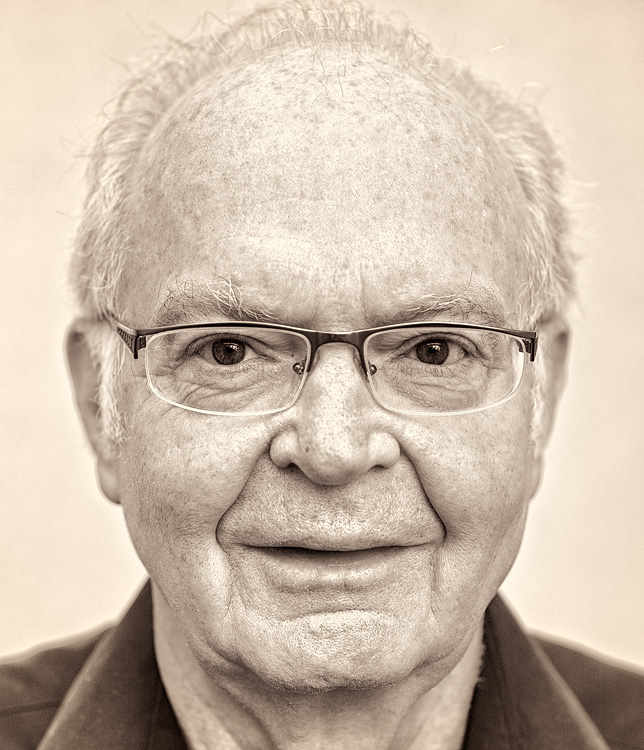
\includegraphics[height=0.6\linewidth]{images/Donald-Knuth-Stanford-Computer-Science}
			\caption{Donald Ervin Knuth. Creador de \TeX}
			\label{fig:donald-knuth-stanford-computer-science}
		\end{figure}
		\end{verbatim}
	\end{block}
	\begin{block}{}
		$\bullet$ \verb|\includegraphics[keyvals]{imagefile}| [Keyvals] son los valores de tamaño; se está haciendo aritmética, se esta cogiendo el 0.6 de todo el tamaño de línea. \{Dirección relativa a la imagen desde nuestro archivo\} \\
		$\bullet$ \verb|\caption{text}| Nota a pie de imagen \\
		$\bullet$ \verb|\label{key}| Referencia a la imagen, muy usada en textos científicos
	\end{block}
\end{frame}

\subsection{Items, enumeraciones y pie de página}

\begin{frame}[fragile]
	\begin{block}{Items}
		\verb|\begin{itemize}| \\
		\verb|\item[label] description| \\
		\verb|\end{itemize}| 
	\end{block}
	\begin{block}{Enumerate}
		\verb|\begin{enumerate}| \\
		\verb|\item[label] description| \\
		\verb|\end{enumerate}|
	\end{block}
	\begin{block}{Notas a pie de página}
		Esto es un poco de texto.\footnote{Y esto la anotación} Y este mejor\footnote[frame]{¿A que sí?} \\~
		
		\verb|Esto es un poco de texto.\footnote{Y esto la anotación}| \\
		\verb|Y este mejor\footnote[frame]{¿A que sí?}|
	\end{block}
\end{frame}

\section{Datos importantes no cubiertos}

\begin{frame}[fragile]
	\frametitle{Datos no cubiertos que se recomienda leer}
	\begin{block}{}
		\begin{itemize}
			\item \verb|\begin{verbatim}|
			\item \verb|\makeindex|
			\item \verb|\label{text}|
			\item Bib\LaTeX, una de las herramientas más potentes y queridas. Hace bibliografías y referencias, muy muy bueno y potente, además de elegante
			\item \verb|\begin{wrap*}|
			\item \verb|\begin{...*}|
			\item Romper contadores
			\item Más fuentes (\texttt{avant, bookman, charter, utopia, palatino...})
		\end{itemize}
	\end{block}
\end{frame}

\begin{frame}[plain, c]
	\centering \Huge FIN \\~
	
	Espero veros en la de Beamer y escritura científica
\end{frame}

\begin{frame}
	\frametitle{Recursos y links}
	\centering \Huge Dudas
	\normalsize
	\begin{block}{}
		\href{https://www.overleaf.com/}{\textbf{Overleaf:}} escritura de \LaTeX\ on-line \\
		\href{http://www.texstudio.org/}{\textbf{\TeX Studio:}} editor usado
	\end{block}
	\begin{block}{}
		\href{https://tobi.oetiker.ch/lshort/lshort.pdf}{\textbf{Libro:} \textit{The not so Short Introduction to \LaTeX}} \\
		\textbf{Correo:} 201507027@alu.comillas.edu
	\end{block}
\end{frame}

\end{document} 